\documentclass{beamer}
\mode<presentation>
{
  \usepackage{theme/theme}
  \setbeamercovered{transparent}
}

\usepackage{amsmath,amssymb,amsfonts}
\usepackage{times}
\usepackage{graphicx}
\usepackage{fancyvrb}
\usepackage{array}
\usepackage{colortbl}
\usepackage{tabularx}
\usepackage{fontspec}
\usepackage{minted}

% Uncomment me when you need to insert code
\usepackage{color}
\usepackage{listings}
% End Code

% End Header

% Titlepage
\newcommand{\maintitle}{T6. Web Presentation Patterns}
\title{\maintitle}
\author{Enterprise Software Architectures}
\institute
{
  Bachelor's Degree in Computer Engineering
}
\date{Academic year 2025/26}
% End Titlepage

\AtBeginSection[]{
  \begin{frame}
    \centering
    \begin{beamercolorbox}[sep=8pt,center]{title}
      \usebeamerfont{title}\insertsectionhead
    \end{beamercolorbox}
  \end{frame}
}

% Slides
\begin{document}

\begin{frame}
  \titlepage
\end{frame}

\begin{frame}
  \frametitle{\maintitle}
  \tableofcontents[subsectionstyle=show]
\end{frame}

\section{Block A - Web Presentation Patterns}

\subsection{Model-View-Controller (MVC)}
\begin{frame}
  \frametitle{Model-View-Controller (MVC)}

  \begin{columns}
    \column{0.6\textwidth}
    Architectural pattern for \textbf{separating concerns} in user interfaces (web-based or otherwise).
    \newline

    Created in the 1970s at Xerox PARC for the Smalltalk programming language.

    \column{0.4\textwidth}
    \centering
    \begin{figure}
      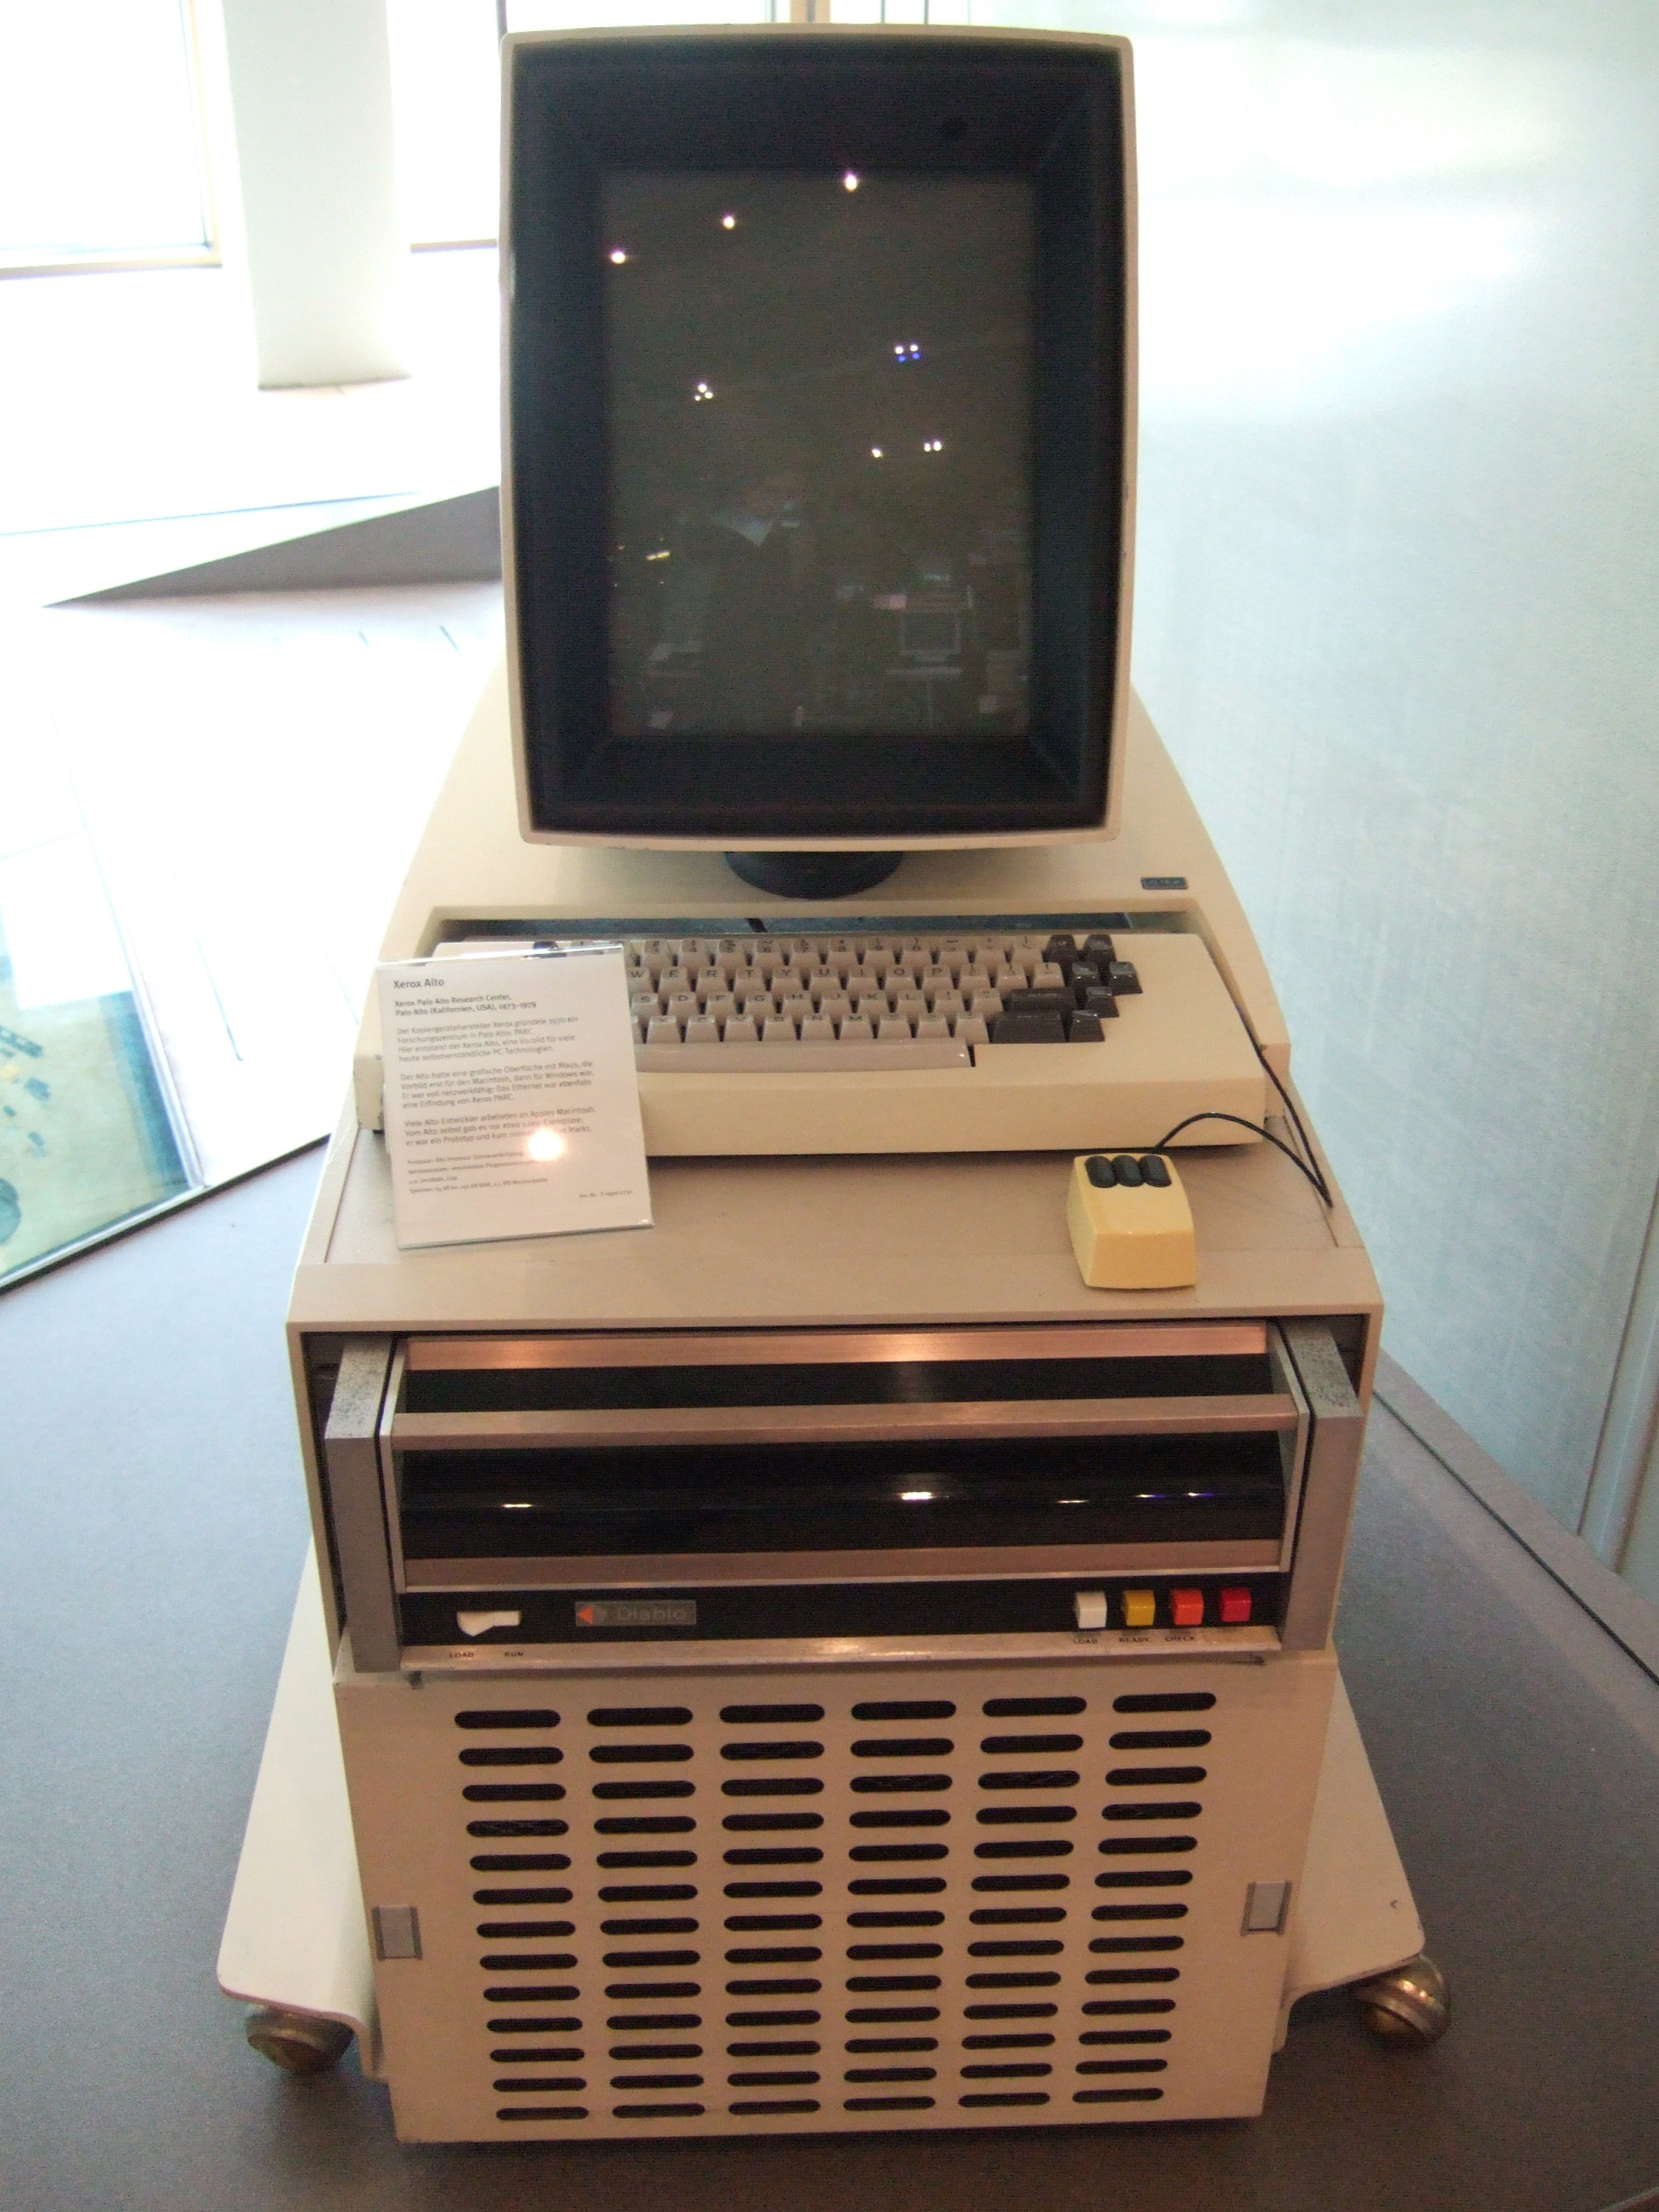
\includegraphics[height=0.6\textheight]{images/T6/xerox-alto.png}
      \caption{Xerox Alto (1973). Source: \href{https://commons.wikimedia.org/wiki/File:Xerox_Alto_mit_Rechner.JPG}{Wikimedia Commons}}
    \end{figure}
  \end{columns}

\end{frame}

\begin{frame}
  \frametitle{Model-View-Controller (MVC)}

  \begin{columns}
    \column{0.5\textwidth}
    \begin{itemize}
      \item \textbf{Model}: Encapsulates business logic and data. Unaware of the UI.
      \item \textbf{View}: Renders the UI using data from the Model. Unaware of business logic.
      \item \textbf{Controller}: Handles user input and coordinates the Model and View.
    \end{itemize}

    \column{0.45\textwidth}
    \centering
    \begin{figure}
      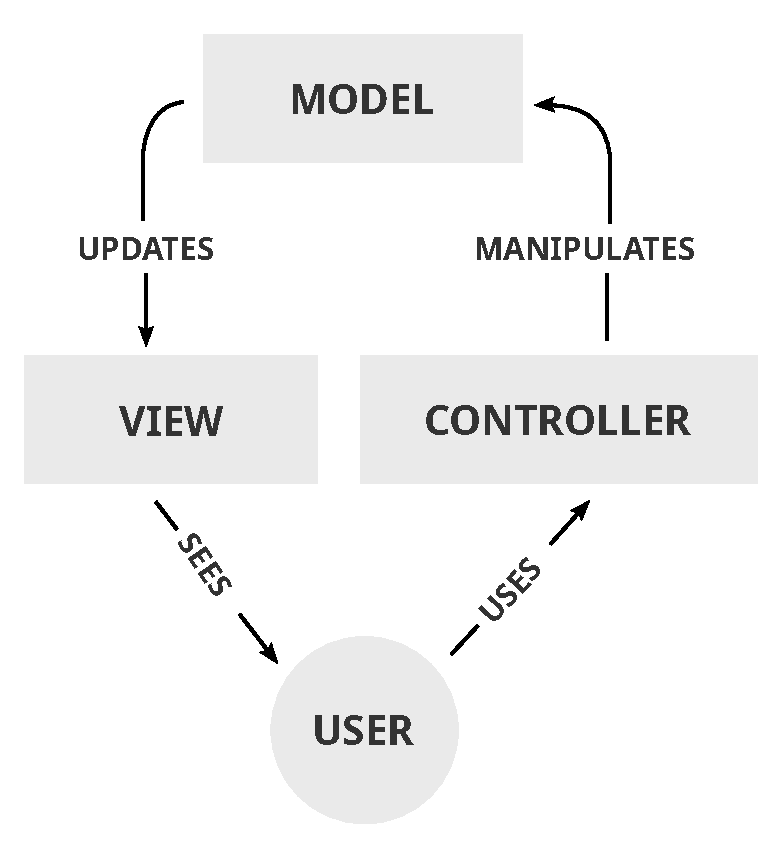
\includegraphics[height=0.6\textheight]{images/T6/mvc-diagram.pdf}
      \caption{MVC pattern overview. Source: \href{https://commons.wikimedia.org/wiki/File:MVC-Process.svg}{Wikimedia Commons}}
    \end{figure}
  \end{columns}

\end{frame}

\begin{frame}
  \frametitle{MVC in a web application}

  In a typical web application, the flow is:

  \begin{enumerate}
    \item The user sends an \textbf{HTTP request} to the Controller.
    \item The Controller interacts with the \textbf{Model} (reads/writes data, executes business logic).
    \item The Controller selects a \textbf{View} and passes the relevant data to it.
    \item The View \textbf{renders} the HTML response that is sent back to the browser.
  \end{enumerate}

\end{frame}

\begin{frame}
  \frametitle{MVC in a web application}

  \centering
  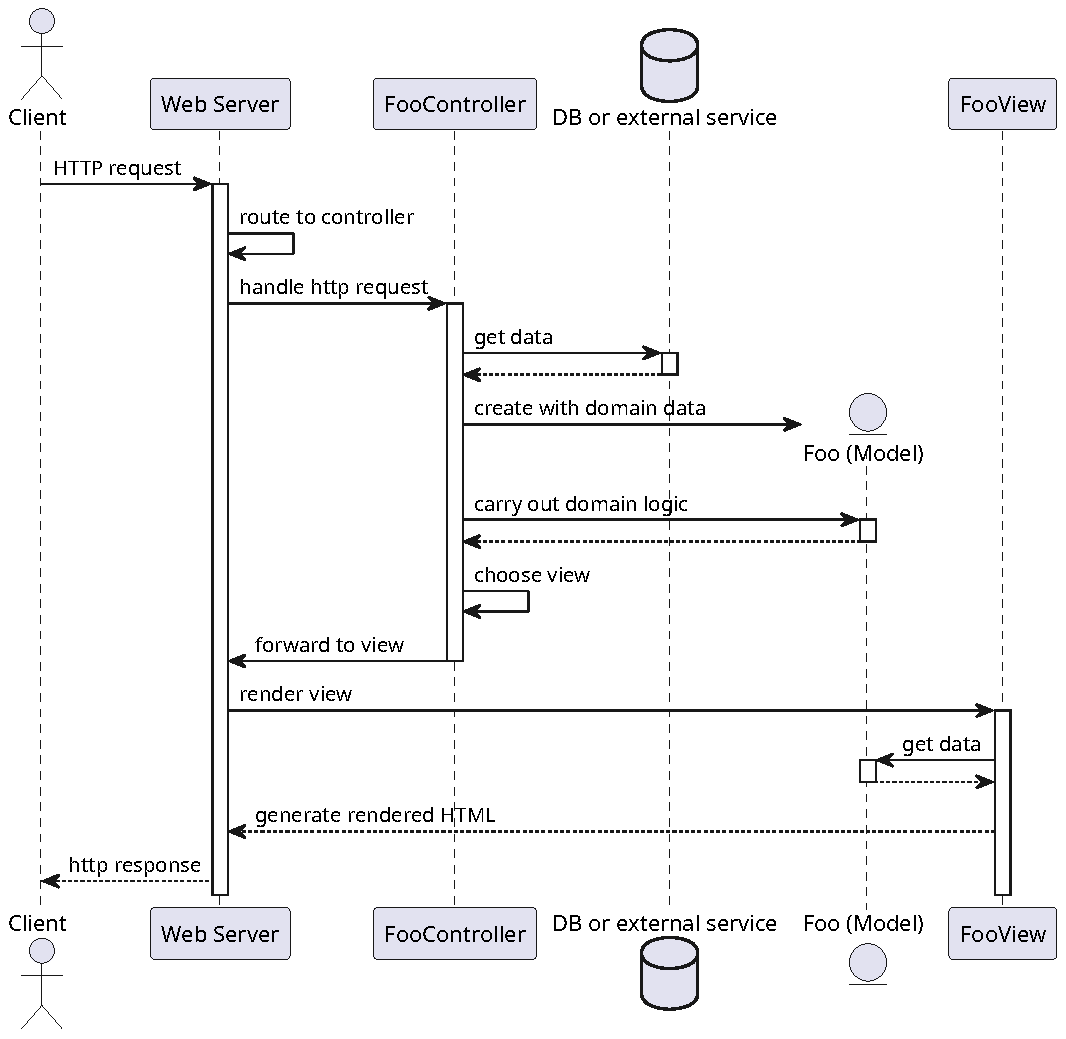
\includegraphics[height=0.8\textheight]{images/T6/mvc-sequence.pdf}

\end{frame}

\subsection{MVC Variants}

\begin{frame}
  \frametitle{MVC variants}

  Several variants of MVC have been proposed to address specific design trade-offs:

  \begin{itemize}
    \item \textbf{Model-View-Adapter (MVA)}: The View does not know of the Model's existence. The Adapter acts as a translation layer, adapting data to the View's needs.
    \item \textbf{Model-View-Presenter (MVP)}: Similar to MVA, but most of the View's logic is delegated to the Presenter.
    \item \textbf{Model-View-ViewModel (MVVM)}\footnote{The MVVM pattern has inspired several modern frontend frameworks, such as Angular and React.}: The ViewModel exposes observable state that the View binds to declaratively. Also known as \textit{Presentation Model}.
  \end{itemize}

\end{frame}

\subsection{View Patterns}

\begin{frame}
  \frametitle{View patterns}

  Once we have an MVC structure, we still need to decide \textbf{how to implement the View}.
  Two classical patterns exist for this:

  \begin{itemize}
    \item \textbf{Template View}: An almost-HTML page structure that mixes \textit{static markup} with
      \textit{executable code snippets} for dynamic content.
    \item \textbf{Transform View}: A function or component that receives the Model as input
      and \textit{transforms} it into HTML output.
  \end{itemize}

\end{frame}

\begin{frame}
  \frametitle{Template View}

  It's an HTML page with \textit{markers} or \textit{scriptlets} that are replaced with dynamic content at render time.
  \newline
  
  \textbf{Advantages:}
  \begin{itemize}
    \item Easy and fast to develop.
    \item The template closely resembles the final HTML output.
  \end{itemize}
  \textbf{Disadvantages:}
  \begin{itemize}
    \item Mixing markup and code makes templates harder to read, test, and maintain as complexity grows.
  \end{itemize}

\end{frame}

\begin{frame}[fragile]
  \frametitle{Template View | PHP example}

  \begin{minted}[fontsize=\small]{php}
<html>
<body>
  <?php $user = getUserFromDatabase(); ?>
  <h1><?= htmlspecialchars($user->getName()) ?></h1>
  <p>Email: <?= htmlspecialchars($user->getEmail()) ?></p>
  <ul>
    <?php foreach ($user->getPosts() as $post): ?>
      <li><?= htmlspecialchars($post->getTitle()) ?></li>
    <?php endforeach; ?>
  </ul>
</body>
</html>
  \end{minted}

  \begin{itemize}
    \item The PHP code is \textbf{embedded inline} inside the HTML markup.
  \end{itemize}

\end{frame}

\begin{frame}
  \frametitle{Transform View}

  A \textbf{Transform View} is a function (or class) that receives a Model object as argument
  and \textit{returns} HTML output.

  \begin{itemize}
    \item The rendering logic lives \textbf{entirely in code}, not in a template.
    \item \textbf{Advantage}: cleaner separation; the view logic is easy to unit-test.
    \item \textbf{Disadvantage}: generating complex HTML purely in code can become verbose.
  \end{itemize}

\end{frame}

\begin{frame}[fragile]
  \frametitle{Transform View | Raw JavaScript example}

  \begin{minted}[fontsize=\small]{react}
function renderUserProfile(user) {
    return `
        <div class="profile">
            <h1>${escapeHtml(user.name)}</h1>
            <p>Email: ${escapeHtml(user.email)}</p>
            <ul>
                ${user.posts.map(
                  p => `<li>${escapeHtml(p.title)}</li>`
                ).join('')}
            </ul>
        </div>
    `;
}
  \end{minted}

  \begin{itemize}
    \item The Model is an \textbf{argument} to a function that returns HTML.
  \end{itemize}

\end{frame}

\begin{frame}[fragile]
  \frametitle{Transform View | JavaScript + JSX example}

  \begin{minted}[fontsize=\small]{react}
function UserProfile({ user }) {
    return (
        <div className="profile">
            <h1>{user.name}</h1>
            <p>Email: {user.email}</p>
            <ul>
                {user.posts.map(p => (
                    <li key={p.id}>{p.title}</li>
                ))}
            </ul>
        </div>
    );
}
  \end{minted}

  \begin{itemize}
    \item Conceptually, this is identical to the previous example.
  \end{itemize}

\end{frame}


\section{Block B - Rendering Strategies}

\begin{frame}
  \frametitle{Rendering strategies}

  Where and when is the HTML generated?

  \begin{itemize}
    \item \textbf{Static Site Generation (SSG)}: HTML is generated \textit{at build time}.
    \item \textbf{Server-Side Rendering (SSR)}: HTML is generated \textit{on the server} for
      each request.
    \item \textbf{Client-Side Rendering (CSR)}: HTML is generated \textit{in the browser} by JavaScript after the page loads.
    \item \textbf{SSR with Hydration}: SSR for the first load, then CSR takes over for subsequent interactions.
  \end{itemize}

  Each strategy has different trade-offs in terms of \textbf{performance},
  \textbf{SEO}, \textbf{infrastructure complexity}, and \textbf{interactivity}.

\end{frame}

\subsection{Static Site Generation (SSG)}
\begin{frame}
  \frametitle{Static Site Generation (SSG) | Build time}

  \centering
  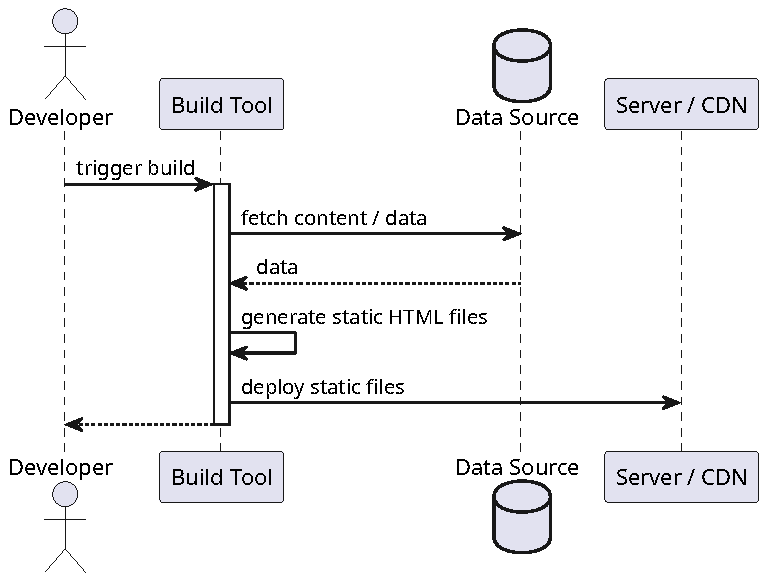
\includegraphics[height=0.75\textheight]{images/T6/ssg-sequence-1.pdf}

\end{frame}

\begin{frame}
  \frametitle{Static Site Generation (SSG) | Request time}

  \centering
  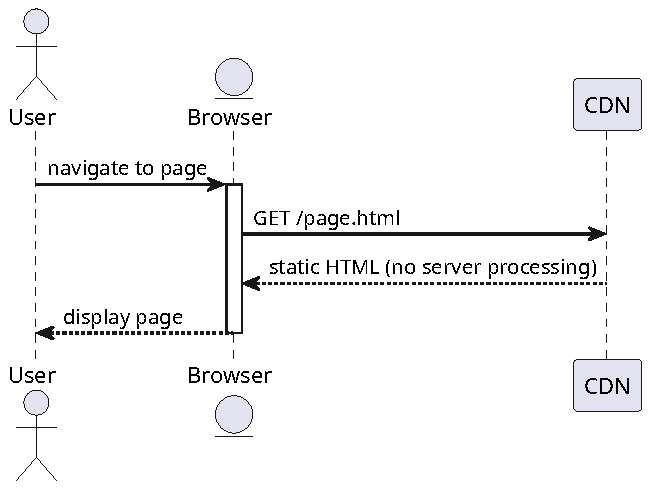
\includegraphics[height=0.7\textheight]{images/T6/ssg-sequence-2.pdf}

\end{frame}

\begin{frame}
  \frametitle{Static Site Generation (SSG)}

  \textbf{Advantages:}
  \begin{itemize}
    \item Extremely fast load times (served from CDN edge).
    \item Cheap (or free) to host.
    \item Great SEO: full HTML available to crawlers.
  \end{itemize}
  \textbf{Disadvantages:}
  \begin{itemize}
    \item Content is \textbf{stale} until the next build.
    \item Not suitable for highly dynamic or personalised content.
    \item Large sites can have long build times.
  \end{itemize}

  \begin{block}{Typical use cases}
    Blogs, documentation sites, marketing pages...
  \end{block}

\end{frame}

\subsection{Server-Side Rendering (SSR)}
\begin{frame}
  \frametitle{Server-Side Rendering (SSR)}
  \centering
  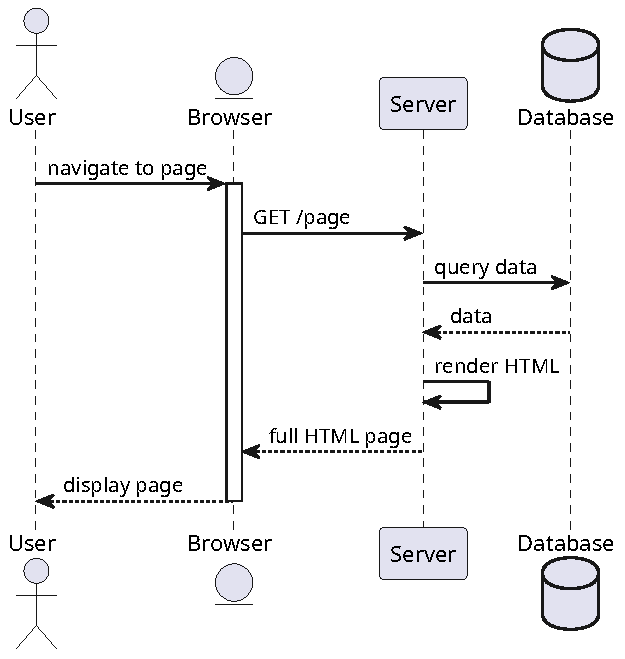
\includegraphics[height=0.85\textheight]{images/T6/ssr-sequence.pdf}
\end{frame}

\begin{frame}
  \frametitle{Server-Side Rendering (SSR)}

  \textbf{Advantages:}
  \begin{itemize}
    \item Content is always \textbf{up to date}.
    \item Good SEO.
    \item Supports personalised content per user.
  \end{itemize}
  \textbf{Disadvantages:}
  \begin{itemize}
    \item High server load and infrastructure cost.
    \item Slower than SSG (a full render on every request).
    \item Latency depends on server and DB response time.
  \end{itemize}

  \begin{block}{Typical use cases}
    News sites, e-commerce sites...
  \end{block}

\end{frame}


\subsection{Client-Side Rendering (CSR)}
\begin{frame}
  \frametitle{Client-Side Rendering (CSR)}
  \centering
  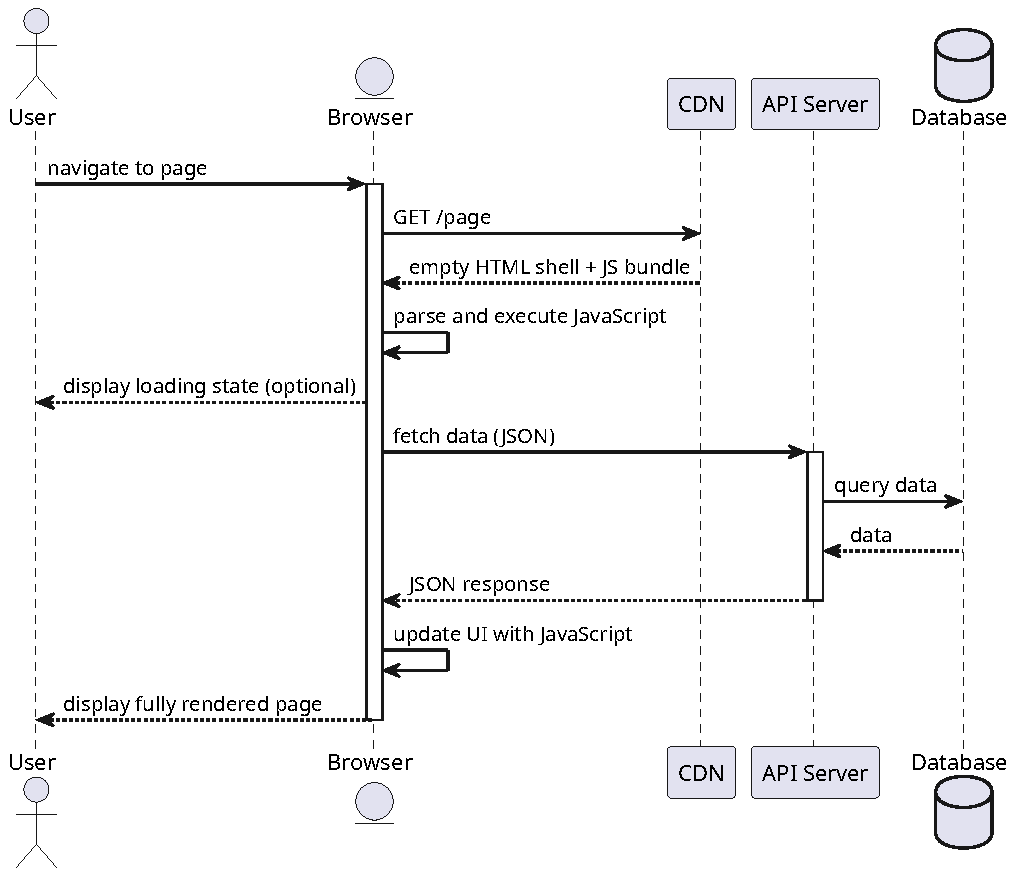
\includegraphics[height=0.85\textheight]{images/T6/csr-sequence.pdf}
\end{frame}

\begin{frame}
  \frametitle{Client-Side Rendering (CSR)}

  \textbf{Advantages:}
  \begin{itemize}
    \item Rich, highly interactive UX.
    \item Reduced server load after initial load.
    \item Fast page transitions (no full page reload).
  \end{itemize}
  \textbf{Disadvantages:}
  \begin{itemize}
    \item Slow initial load (\textit{Time to First Contentful Paint}).
    \item Poor SEO without additional workarounds.
  \end{itemize}

  \begin{block}{Typical use cases}
    Web-apps, dashboards, admin panels...
  \end{block}

\end{frame}


\subsection{SSR with Hydration}
\begin{frame}
  \frametitle{SSR with Hydration}
  \centering
  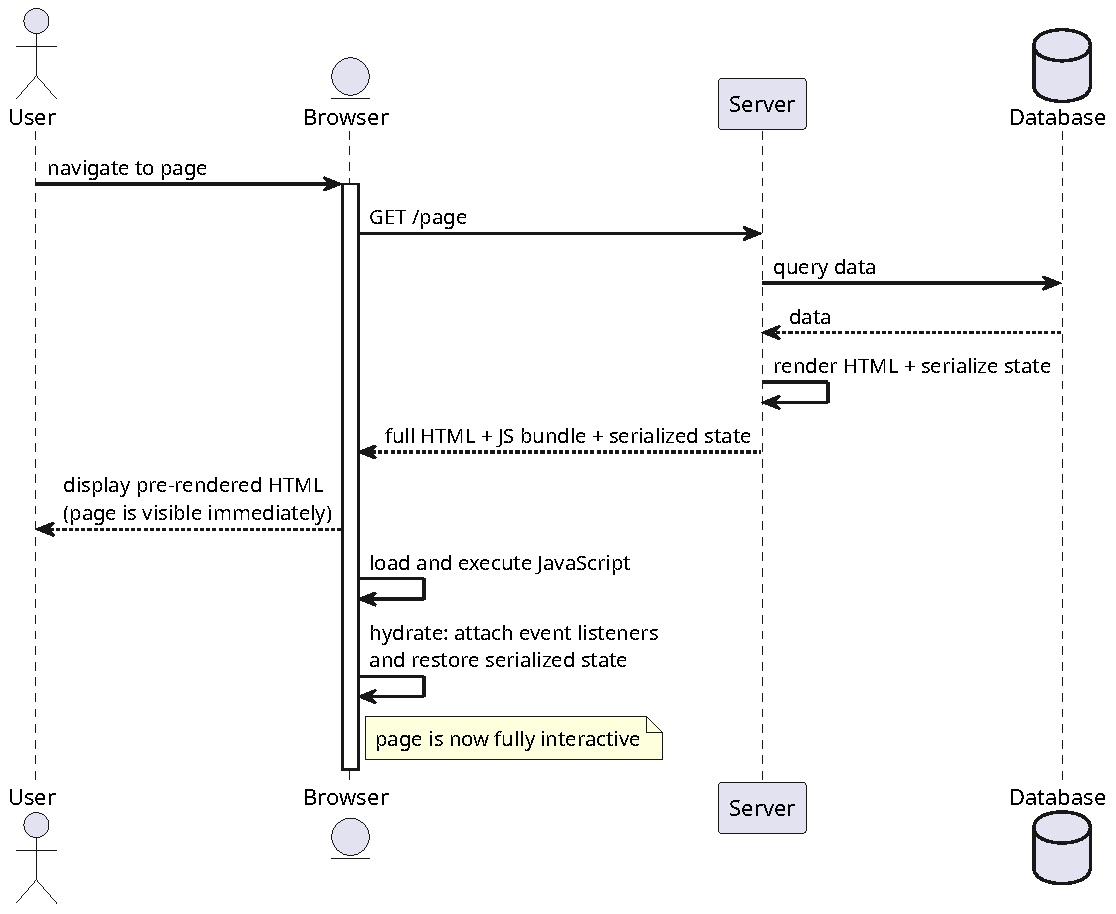
\includegraphics[height=0.85\textheight]{images/T6/hydration-sequence.pdf}
\end{frame}

\begin{frame}
  \frametitle{SSR with Hydration}

  \textbf{Advantages:}
  \begin{itemize}
    \item Fast \textit{Time to First Contentful Paint} (SSR benefit).
    \item Good SEO (SSR benefit).
    \item Full interactivity after hydration (CSR benefit).
  \end{itemize}
  \textbf{Disadvantages:}
  \begin{itemize}
    \item Most complex to implement.
    \item Page is visible but \textbf{not interactive} until JS is loaded
      (\textit{Time to Interactive} gap).
    \item Higher server load than pure CSR.
  \end{itemize}

\end{frame}


\newcommand{\colGood}[1]{\textbf{\textcolor{green!60!black}{#1}}}
\newcommand{\colMid}[1]{\textbf{\textcolor{orange!80!black}{#1}}}
\newcommand{\colBad}[1]{\textbf{\textcolor{red!70!black}{#1}}}

\begin{frame}

  \frametitle{Rendering strategies comparison}

  \begin{tabularx}{\textwidth}{l X X X X}
    \hline
    & \textbf{SSG} & \textbf{SSR} & \textbf{CSR} & \textbf{Hydration} \\
    \hline
    Dynamic data   & \colBad{No}       & \colGood{Yes}     & \colGood{Yes}     & \colGood{Yes}   \\
    First paint    & \colGood{Fast}    & \colMid{Medium}   & \colBad{Slow}     & \colMid{Medium} \\
    Interactivity  & \colBad{Low}      & \colMid{Medium}   & \colGood{High}    & \colGood{High}  \\
    SEO            & \colGood{Great}   & \colGood{Good}    & \colBad{Poor}     & \colGood{Good}  \\
    Server cost    & \colGood{Minimal} & \colBad{High}     & \colGood{Low}     & \colMid{Medium} \\
    Complexity     & \colGood{Low}     & \colMid{Medium}   & \colMid{Medium}   & \colBad{High}   \\
    \hline
  \end{tabularx}

\end{frame}

\end{document}
